\documentclass[10pt, letterpaper]{report}
% !TeX program = xelatex
%==================PREAMBOLO=======================%
\usepackage[utf8]{inputenc}
\usepackage{psvectorian}
\usepackage{pgfplots}
\usepackage[Rejne]{fncychap}
\usepackage[export]{adjustbox}
\usepackage[T1]{fontenc}
\usepackage{lmodern}
\usepackage{blindtext}
\usepackage{pdfpages}
\usepackage[shortlabels]{enumitem}
\usepackage{moresize}
\usepackage{graphicx} % Required for inserting images
\usepackage{hyperref}
\usepackage{listings}
\usepackage[table,xcdraw]{xcolor}
\usepackage{amssymb}
\usepackage{amsmath}
\usepackage[english]{babel}
\usepackage{nicefrac, xfrac}
\usepackage{tikz}
\usepackage{tikz-3dplot}
\usepackage{tikz-cd}
\usepackage{mathrsfs} 
\usepackage{titletoc}
\usepackage{fancyhdr}
\usepackage{psvectorian,lipsum}
\usepackage{fourier-orns}
\usepackage{lipsum}
\usepackage{wrapfig}
\usepackage{multicol}
\usepackage[paper=a4paper,left=25mm,right=25mm,bottom=25mm,top=25mm]{geometry}
\definecolor{light-gray}{gray}{0.95}
\definecolor{cop}{HTML}{f7ecd7}
\definecolor{copAut}{HTML}{ababab}
\definecolor{copAut2}{HTML}{c3c3e6}
\definecolor{purcop}{HTML}{d0d3db}
\definecolor{sapienza}{HTML}{660f1d}
\definecolor{lightSapienza}{HTML}{e3d3d5}
\definecolor{darkgreen}{HTML}{008000}
\definecolor{cartaRiciclata}{HTML}{fcfcf7}
\newcommand{\redText}[1]{\color{red}#1\color{black}}
\newcommand{\code}[1]{\colorbox{light-gray}{\texttt{#1}}}
\newcommand{\codee}[1]{\colorbox{white}{\texttt{#1}}}
\newcommand{\K}{{\mathbb K}}
\newcommand{\notimplies}{%
  \mathrel{{\ooalign{\hidewidth$\not\phantom{=}$\hidewidth\cr$\implies$}}}}
\newcommand{\flowerLine}{ \begin{center}\decofourleft\hphantom{ }\decoone\hphantom{ }\decofourright\hphantom{}\hphantom{aa}
\decofourleft\hphantom{ }\decoone\hphantom{ }\decofourright\hphantom{}\hphantom{aa}
\decofourleft\hphantom{ }\decoone\hphantom{ }\decofourright\hphantom{}\hphantom{aa}
\decofourleft\hphantom{ }\decoone\hphantom{ }\decofourright\hphantom{}\hphantom{aa} 
\decofourleft\hphantom{ }\decoone\hphantom{ }\decofourright\hphantom{}\hphantom{aa}
\decofourleft\hphantom{ }\decoone\hphantom{ }\decofourright\hphantom{}\hphantom{aa}
\decofourleft\hphantom{ }\decoone\hphantom{ }\decofourright\hphantom{}\hphantom{aa}
\decofourleft\hphantom{ }\decoone\hphantom{ }\decofourright\hphantom{}\hphantom{aa}
\decofourleft\hphantom{ }\decoone\hphantom{ }\decofourright\hphantom{}\hphantom{aa}
\end{center}}
\definecolor{g}{RGB}{60, 50, 50}
\newcommand{\textg}[1]{\color{g}{\textbf{#1}}\color{black}}
\newcommand{\teo}[1]{{\large\color{sapienza}\textbf{Teorema #1 :\hphantom{a}}}}
\newcommand{\defi}[1]{{\large\color{sapienza}\textbf{Definizione #1 :\hphantom{a}}}}
\newcommand{\claim}[1]{{\color{sapienza}\textbf{Claim #1 :\hphantom{a}}}}
\newcommand{\lemma}[1]{{\color{sapienza}\textbf{Lemma #1 :\hphantom{a}}}}
\newcommand{\dimo}[1]{{\color{sapienza}\textbf{Dimostrazione #1 :\hphantom{a}}}}
\newcommand{\prop}[1]{{\color{sapienza}\textbf{Proposizione #1 :\hphantom{a}}}}
\newcommand\greybox[1]{%
  \vskip\baselineskip%
  \par\noindent\colorbox{light-gray}{%
    \begin{minipage}{\textwidth}#1\end{minipage}%
  }%
  \vskip\baselineskip%
}
\newcommand\sapbox[1]{%
  \vskip\baselineskip%
  \par\noindent\colorbox{lightSapienza}{%
    \begin{minipage}{\textwidth}#1\end{minipage}%
  }%
  \vskip\baselineskip%
}
\newcommand{\ridFunc}{{f:\Sigma^*\rightarrow \Sigma^*}}
\newcommand{\rid}{{\le_m^P}}
\newcommand{\Z}{{\mathbb Z}}
\newcommand{\blank}{{\sqcup}}
\newcommand{\Prob}{{\mathbb P}}
\newcommand{\R}{{\mathbb R}}
\newcommand{\VA}{{\mathbb E}}
\newcommand{\N}{{\mathbb N}}
\newcommand{\quat}{{\mathbb H}}
\newcommand{\C}{{\mathbb C}}
\newcommand{\Sn}{{\mathcal S_n}}
\newcommand{\An}{{\mathcal A_n}}
\newcommand{\E}{{\mathcal E}}
\newcommand{\B}{{\mathcal B}}
\newcommand{\mcm}{{\text{mcm}}}
\newcommand{\rg}{{\text{rg}}}
\newcommand{\ve}{{\bar v}}
\newcommand{\spaz}{{\text{\hphantom{aa}}}}
\newcommand{\MCD}{{\text{MCD}}}
\newcommand{\tc}{{\text{ tale che }}}
\newcommand{\supp}{{\text{Supp}}}
\newcommand{\acc}{\\\hphantom{}\\}
\newcommand{\esempio}[1]{{\acc\large\color{sapienza}\textbf{Esempio #1 \hphantom{a}}\acc}}
\newcommand{\bra}[1]{\langle #1 \rangle}
\newcommand{\aut}{{\text{Aut}}}
\newcommand{\Span}{{\text{Span}}}
\newcommand{\End}{{\text{End}}}
\newcommand{\cen}{{\text{Centro}}}
\newcommand{\norm}{{\unlhd}}
\newcommand{\ciclS}{{\left \langle }}
\newcommand{\ciclE}{{\right \rangle }}
\newcommand{\boxedMath}[1]{\begin{tabular}{|c|}\hline \texttt{#1} \\ \hline\end{tabular} :} 
\newcommand{\shell}[1]{\colorbox{black}{\textcolor{white}{\texttt{#1}}}}
\newcommand{\eqImportante}[1]{\begin{center}\huge\lefthand\hphantom{a}
    \normalsize\texttt{#1}
    \hphantom{aaa}\huge\righthand\end{center}}

\fancyhf{}
\pagestyle{fancy}
\usepackage{pgf-pie}  
\usetikzlibrary{positioning}

\renewcommand{\headrule}{%
\vspace{-8pt}\hrulefill
\raisebox{-2.1pt}{\quad\decothreeleft\decotwo\decothreeright\quad}\hrulefill}

%sta roba serve per il codice C
\definecolor{mGreen}{rgb}{0,0.6,0}
\definecolor{mGray}{rgb}{0.5,0.5,0.5}
\definecolor{mPurple}{rgb}{0.58,0,0.82}
\definecolor{backgroundColour}{rgb}{0.95,0.95,0.92}

\lstdefinestyle{CStyle}{
    backgroundcolor=\color{backgroundColour},   
    commentstyle=\color{mGreen},
    keywordstyle=\color{magenta},
    numberstyle=\tiny\color{mGray},
    stringstyle=\color{mPurple},
    basicstyle=\footnotesize,
    breakatwhitespace=false,         
    breaklines=true,                 
    captionpos=b,                    
    keepspaces=true,                 
    numbers=left,                    
    numbersep=5pt,                  
    showspaces=false,                
    showstringspaces=false,
    showtabs=false,                  
    tabsize=2,
    language=C
}
\lstdefinestyle{CppStyle}{
    backgroundcolor=\color{backgroundColour},   
    commentstyle=\color{mGreen}\ttfamily,
    morecomment=[l][\color{magenta}]{\#}
    keywordstyle=\color{blue}\ttfamily,
    numberstyle=\tiny\color{mGray},
    stringstyle=\color{red}\ttfamily,
    basicstyle=\ttfamily,
    breakatwhitespace=false,         
    breaklines=true,                 
    captionpos=b,                    
    keepspaces=true,                 
    numbers=left,                    
    numbersep=5pt,                  
    showspaces=false,                
    showstringspaces=false,
    showtabs=false,                  
    tabsize=2,
    language=C
}
\lstset{language=C++,
                basicstyle=\ttfamily,
                keywordstyle=\color{blue}\ttfamily,
                stringstyle=\color{red}\ttfamily,
                commentstyle=\color{green}\ttfamily,
                morecomment=[l][\color{magenta}]{\#}
}
%fine roba che serve per il codice C
\usepackage{minted}
\usepackage{algorithm}
\usepackage{algpseudocode}
\usepackage{booktabs}
\newcommand{\titolo}{Machine Learning }

 %TOGLI COMMENTO SE USI XELATEX
%\usepackage{fontspec}
\title{\titolo} %========TITOLO========%
\author{Marco Casu}
\date{\vspace{-5ex}}
\begin{document}

%==================COPERTINA=======================%
\begin{titlepage}
    
\begin{center}
    %TOGLI COMMENTO SE USI XELATEX
   %\setmainfont{Palace Script MT}
   \HUGE Marco Casu\acc
\end{center}
\thispagestyle{empty}
\begin{figure}[h]
    \centering{
        %l'immagine deve avere una risoluzione 2048x2048
        
\includegraphics[width=1\textwidth ]{images/Copertina.png}
    }
\end{figure}
\vfill 
\centering 
\includegraphics[width=0.4\textwidth ]{../../preamble/Stemma_sapienza.png} \acc
\centering \Large \color{sapienza}Faculty of Information Engineering, Computer Science and Statistics\\
Department of Computer, Control and Management Engineering\\
Master's degree in Artificial Intelligence and Robotics
\end{titlepage}

%===================FINE COPERTINA======================%
\newpage
%\pagecolor{cartaRiciclata}%\setmainfont{Algerian}
\Large
This document summarizes and presents the topics for the \titolo course for the Master's degree in Artificial Intelligence and Robotics at Sapienza University of Rome. The document is free for any use. If the reader notices any typos, they are kindly requested to report them to the author.
\vfill
\begin{figure}[h!]
    \raggedright
    
\includegraphics[width=0.4\textwidth,right ]{../../preamble/tomodachi.pdf} 
\end{figure}
\newpage %\setmainfont{Times New Roman}
\normalsize

\tableofcontents 
\newpage

%==================FOOTER e HEADER=======================%
\fancyhf{}
\fancyhead[L]{\nouppercase{\leftmark}}
\fancyhead[R]{Sezione \thesection}
\fancyfoot[C]{\thepage}
\fancyfoot[L]{\titolo}
\fancyfoot[R]{ Marco Casu}
%\fancyfoot[R]{\setmainfont{Palace Script MT}\huge Marco Casu \setmainfont{Times New Roman}}
%==================FOOTER e HEADER=======================%

\newtheorem{definition}{Definition}

%==================INIZIO======================%
\chapter{Introduction}
\section{Basic Definition of a ML Problem}
In this chapter we will introduce the basics of what is a machine learning problem, giving a mathematical definition. informally, with machine learning we define the use of knowledge (data) to improve the performance of a given program, using past experiences.\bigskip

Generally, we use machine learning to solve problems with no deterministic solutions, trying to find an approximate one (such as recognizing what animal is represented in a given photo).\bigskip 

Usually, a machine learning problem consists in three main component:\begin{itemize}
    \item $T$ : the given task
    \item $P$ : a performance metric
    \item $E$ : the past experiences (the data)
\end{itemize}
Let's see an example, we want to model a program capable of playing \textit{Checkers}.
\begin{center}
    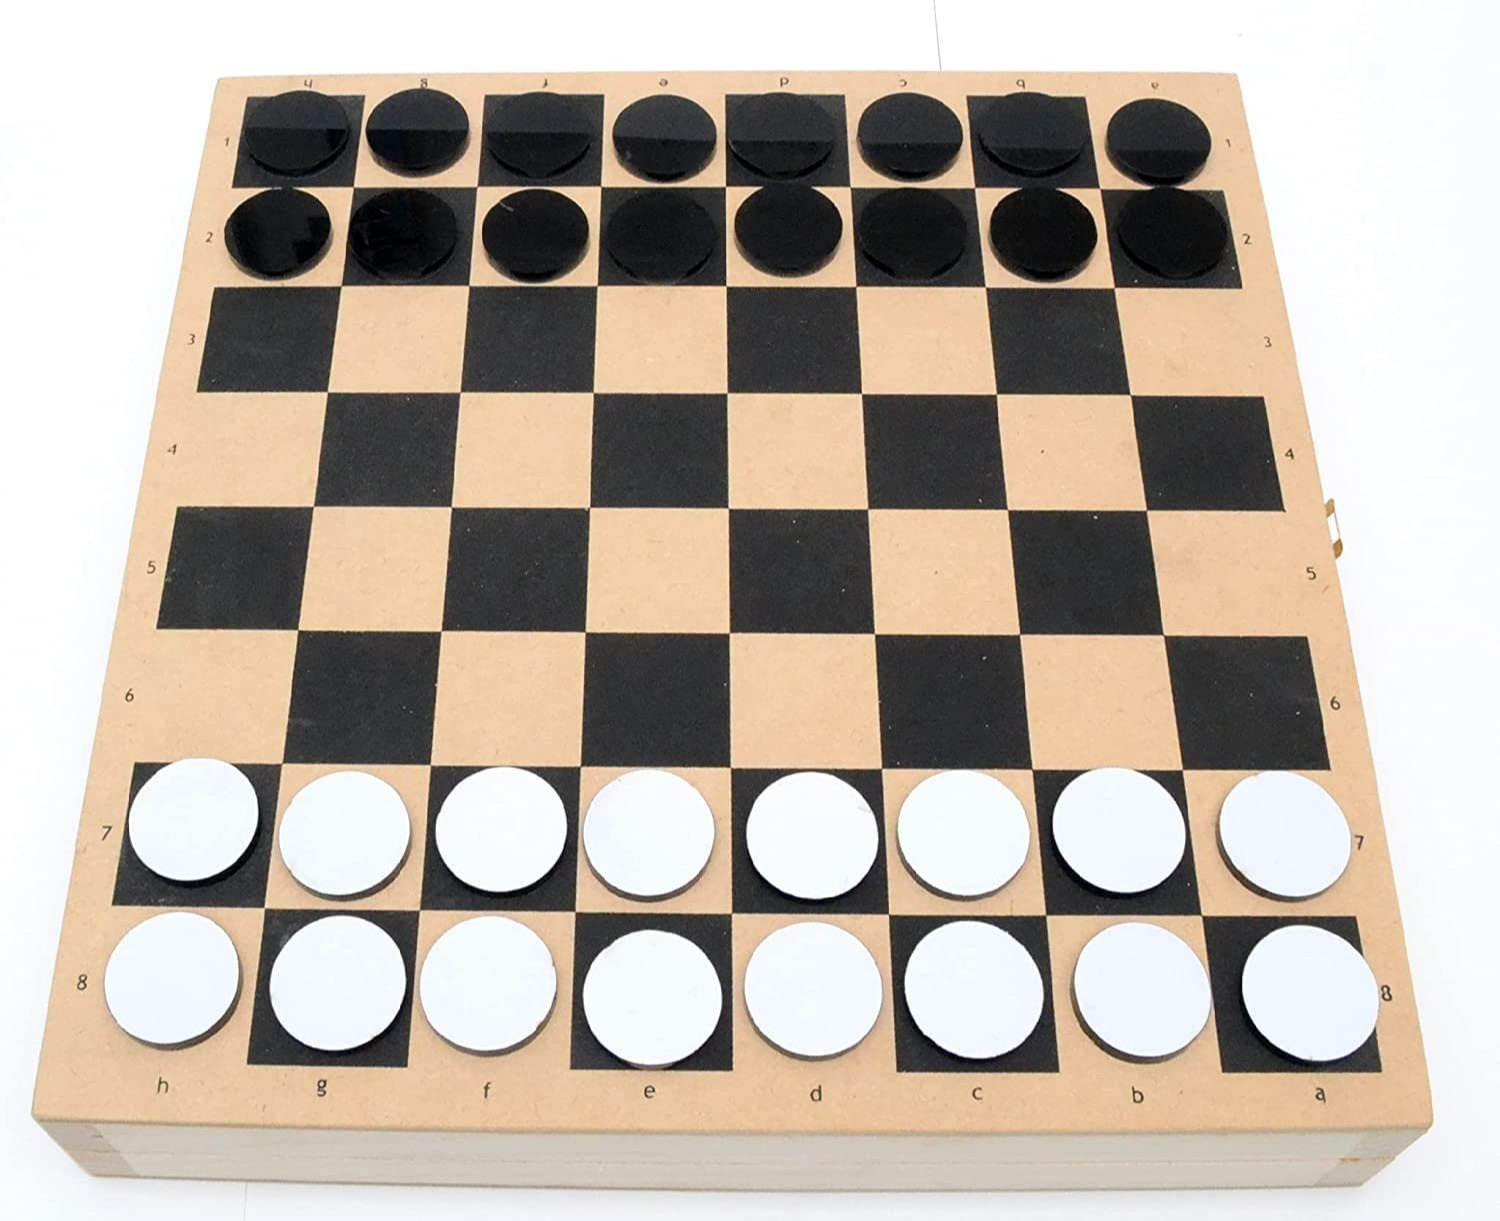
\includegraphics[width=0.35\textwidth]{images/Checkers.jpg}
\end{center}
The task $T$ is to play the game, the performance metric $P$ measure the ratio of win in a tournament, and the experiences is given by the past match. We can create this matches by letting the computer play against himself, or by making it play against a human. We can consider two types of target functions that models the behavior of the model:\begin{itemize}
    \item $ChooseMove : Board\rightarrow Move$
    \item $V : Board\rightarrow\R$
\end{itemize}
$Board$ is the set of the possible board configurations, move is the set of feasible moves. The image of the function $V$ should represents the validity of a board in the following sense:\begin{itemize}
    \item if $b\in Boards$ is a configuration that represents the win of the player, then $V(b)=1$
    \item else if $b\in Boards$ is a configuration that represents the win of the opponent, then $V(b)=-1$
    \item else if $b\in Boards$ is a configuration that represents a draw, then $V(b)=0$
    \item else, $V(b)=V(b')$ where $b'$ is
the best final board state that can be achieved starting from $b$ and
playing optimally until the end of the game.
\end{itemize}
The function $V$ can be used to predict the next move by considering all possible boards that can be obtained from the feasible moves.
We focus on the function $V$, this should be an optimal model, but is not computable, because we cannot tell if a play is ''optimal'' (this is the goal of the model), so we want to consider a function that approximate the behavior of $V$.\bigskip

We consider a function $\hat V: Board\rightarrow\R$ defined as follows:\begin{equation}
    \hat V(b)=\sum_{i=0}^6w_if_i(b)
\end{equation}
where $\mathbf w = (w_i)$ is real coefficients, and the functions $f_i$ represents some features of the given board:\begin{itemize}
    \item $f_1(b)$ : number of black pieces on $b$
    \item $f_2(b)$ : number of red pieces on $b$
    \item ecc...
\end{itemize}
We don't know if some features are useful to predict which move is optimal, is important that this features model the knowledge of the \textit{domain} (in this case, the game of Checkers). \bigskip

with \textit{learning the function} $\hat V$, we intend to finds the coefficients $\mathbf w$ which make the function $\hat V$ more similar to $V$ as possible. There are various method to find these coefficients.\bigskip

Let's introduce some notation:\begin{itemize}
    \item with $V$ we  define the \textbf{target function} (always unknown and uncomputable).
    \item with $\hat V$ we  define the \textbf{learned function}, the approximation of $V$ that we want to find.
    \item with $V_{train}(b)$ we define the value of $V$ obtained at $b$, where $b$ is a part of a data set that is given. We will use the values of $V_{train}$ on the data set to synthesize $\hat V$.
    \item with $D$ we define the given data set:\begin{equation}
        D=\bigcup_{i=1}^n\{(b_i,V_{train}(b_i))\}
    \end{equation}
    $n$ is the number of the available data.
\end{itemize}
The iterative method given in the Algorithm \ref{alg:LMS} is an informal example of how we can find the values for $\mathbf w$.
\begin{algorithm}
    \caption{LMS weight update rule}\label{alg:LMS}
    \begin{algorithmic}
    \Require $D$, $V_{train}$, $k$
    \State initialize $\mathbf w$ with small random values 
    \For{$k$ times}  
    \State select a sample $b$ from $D$
    \State $error(b)=V_{train}(b)-\hat V(b)$
    \For{each feature $i$} 
    \State $w_i\leftarrow w_i+c\cdot f_i(b)\cdot error(b)$
    \EndFor
    \EndFor
    \end{algorithmic}
\end{algorithm}
In this case $c$ is a small constant, usually in $(0,1]$, to moderate the rate of learning.\bigskip

The function $error(b)$ is computable only on the sample $b$ given in the dataset $B$, the goal of the method is to converge to a local minimum for the function  \begin{equation}
    \sum_{b_i\in D}error(b_i).
\end{equation}
Once we synthesize $\hat V$ with this method, we can make the model play against human and track the result to use it as an additional dataset. The diagram in image \ref{img:DesignChoice} represents the process of designing an artificial intelligence agent.

\begin{figure}[h!]
    \centering
    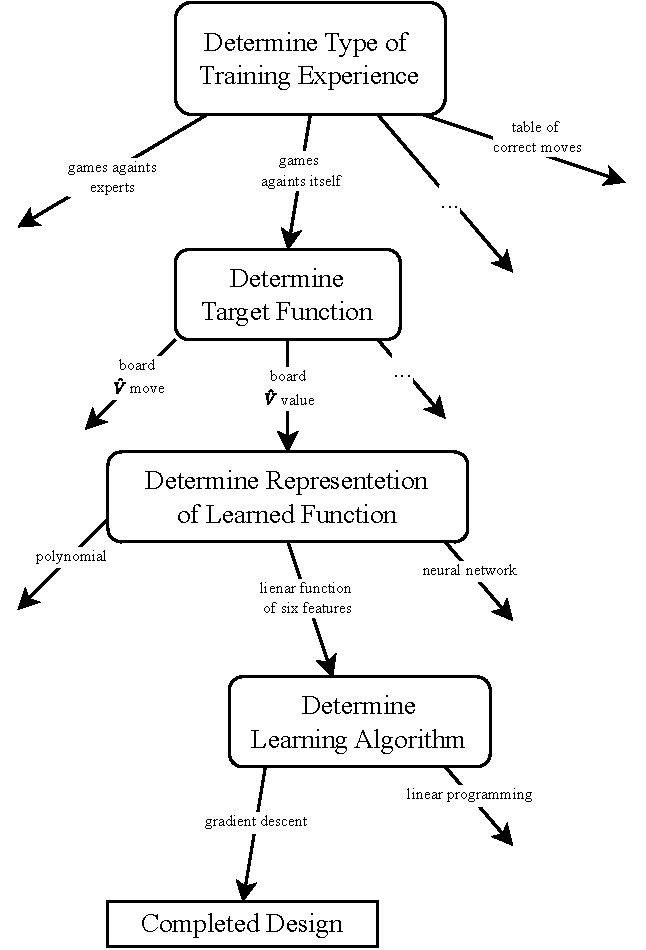
\includegraphics[width=0.35\textwidth]{images/DesignChoice.pdf}
    \caption{Design Choices}
    \label{img:DesignChoice}
\end{figure}
\section{Types of Machine Learning Problems}
There are different types of machine learning problems:\begin{itemize}
    \item Supervised Learning\begin{itemize}
        \item Classification
        \item Regression
    \end{itemize}
    \item Unsupervised Learning
    \item Reinforcement Learning
\end{itemize}

\begin{definition}
    Given a function $f:X\rightarrow Y$, and a training set $X_D\subset X$ containing information about $f$, \textbf{learning} the function $f$ means computing an approximated function $\hat f$ such that is much close as possible to $f$ on $X$\begin{equation}
        \hat f(x)\simeq f(x), \ \ x\in X.
    \end{equation}
\end{definition}
This is not a simple problem, $f$ is not computable, so the difference $f-\hat f$, and $X$ is usually uncountable ora big set, way bigger than the training set $X_D$. \bigskip

Machine learning problems can be classified in terms of the input data set $D$, given a target function $f:X\rightarrow Y$ a problem is\begin{itemize}
    \item a \textbf{supervised learning} problem if $D=\bigcup_{i=1}^n\{(x_i,y_i)\}\subset X\times Y$ .
    \item an \textbf{unsupervised learning} problem if $D=\bigcup_{i=1}^n\{(x_i)\}\subset X$.
    \item a \textbf{reinforcement learning} problem, the condition on the input dataset will be discussed later.
\end{itemize}
The problems can also be classified in terms of the target function $f:X\rightarrow Y$
\begin{align*}
   & X=\begin{cases}
        A_1\times \dots \times A_m, \ A_i \text{ finite set} \ \ \textbf{(Finite Discrete Problem)}\\ 
        \R^n \ \ \textbf{(Continuous)}
    \end{cases}\\ 
    & Y=\begin{cases}
         \R^k \ \ \textbf{(Regression)}\\ 
        \{C_1,C_2\times C_k\} \ \ \textbf{(Classification)}
    \end{cases}
\end{align*}
special case (\textbf{Concept Learning}):\begin{align*}
    & X = A_1\times \dots \times A_m, \ A_i \text{ finite set}\\ 
    & Y = \{0,1\}
\end{align*}
Classification problems is also known as \textit{Pattern Recognition Problems}, the goal is to return the class to which a specific instance belong.\begin{center}
     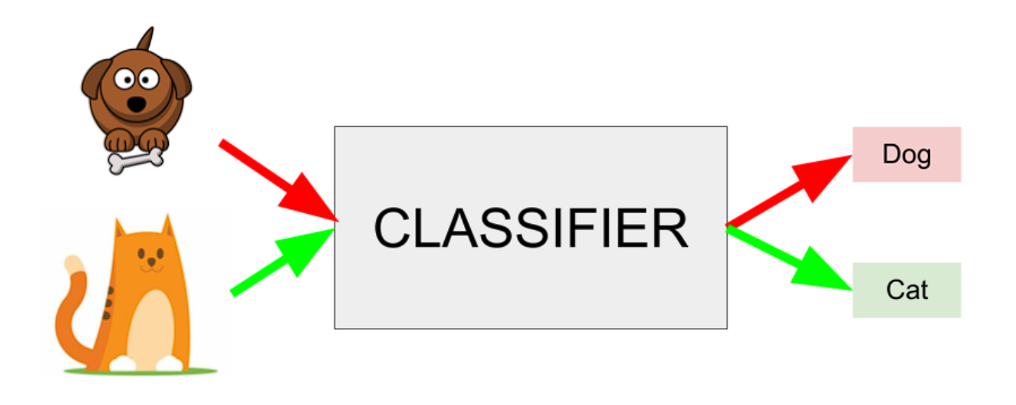
\includegraphics[width=0.6\textwidth]{images/classifier.png}
\end{center}
Some examples are:\begin{itemize}
    \item face/object/character recognition
    \item speech/sound recognition
    \item medical diagnosis
    \item document classification.
\end{itemize}
Regression problems consists in approximating real valued functions.
\begin{center}
     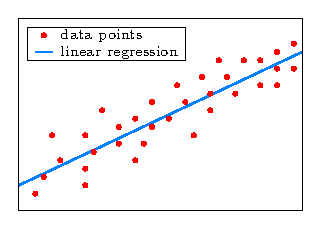
\includegraphics[width=0.35\textwidth]{images/regression.eps}
\end{center}
Unsupervised learning discovers data patterns without a specific output. The main goal is to understand what's normal in a dataset. \textit{Clustering} is a key technique that groups similar data points. Applications include customer segmentation, image compression, and bioinformatics motif learning.\bigskip

Reinforcement learning consists in learning a policy, which is a strategy that tells the agent what action to take in any given situation (or state) to maximize its long-term reward. This is often represented as a function that maps a state to an action. Unlike supervised learning, where the model is trained with labeled examples, in reinforcement learning agents learn through a process of trial and error.\bigskip

They don't have a correct answer to guide them. Instead, they receive sparse and time-delayed rewards. This means the feedback (the reward) for a good action might not come immediately, and it might be a simple, numerical value (like +1 for winning a game or -1 for losing). Some examples are:\begin{itemize}
    \item Game playing: Think of programs that have learned to play chess, Go, or video games better than humans.
    \item Robotic tasks: A robot learning to navigate a room, pick up an object, or perform a specific manufacturing task.
    \item Any dynamical system with an unknown or partially known model: This is a broad category that includes things like optimizing traffic flow, managing a power grid, or controlling financial trading strategies.
\end{itemize}
\begin{center}
     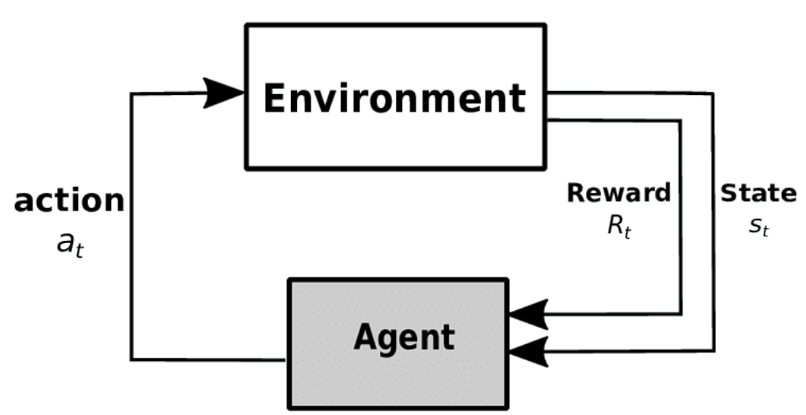
\includegraphics[width=0.35\textwidth]{images/RL_diagram.png}
\end{center}
In concept learning, the output consists in only two classes, the target function $c:X\rightarrow\{0,1\}$ maps  any kind of input in one of two distinct values. The following example model a program that predict if is a good day to play Tennis, the input set is $$ 
X=Day\times Outlook \times Temperature \times Humidity \times Wind 
$$
the output set is $PlayTennis=\{\text{Yes, No}\}$. An example of data samples:\begin{center}
\begin{tabular}{cccccc}
\toprule
$Day$ & $Outlook$ & $Temperature$ & $Humidity$ & $Wind$ & $PlayTennis$ \\
\midrule
D1 & Sunny & Hot & High & Weak & No \\
D2 & Sunny & Hot & High & Strong & No \\
D3 & Overcast & Hot & High & Weak & Yes \\
D4 & Rain & Mild & High & Weak & Yes \\
D5 & Rain & Cool & Normal & Weak & Yes \\
D6 & Rain & Cool & Normal & Strong & No \\
D7 & Overcast & Cool & Normal & Strong & Yes \\
D8 & Sunny & Mild & High & Weak & No \\
D9 & Sunny & Cool & Normal & Weak & Yes \\
D10 & Rain & Mild & Normal & Weak & Yes \\
D11 & Sunny & Mild & Normal & Strong & Yes \\
D12 & Overcast & Mild & High & Strong & Yes \\
D13 & Overcast & Hot & Normal & Weak & Yes \\
D14 & Rain & Mild & High & Strong & No \\
\bottomrule
\end{tabular}
\end{center}
\section{Performance Evaluation}
Usually, we call \textbf{Hypothesis} a possible learned function $h$, and we define $H$ as the \textbf{Hypothesis space}, such space contains all possible function that can be learnt (all possible approximation of the target function). In this terms, a learning problem is described as a search in the hypothesis space using the given dataset $D$, that aims to find the best possible approximation $h^*$:\begin{equation}\label{sol_hypothesis}
    h^*=\arg \max_{h\in H} Performance(h,D)
\end{equation} 
\subsection{Concept Learning}
We focus now on the concept learning (binary classification), let's consider a target function\begin{equation}
    c:X\rightarrow \{0,1\}
\end{equation}
let $D\subset \{X,Y\}$ to be the sample set\begin{equation}
    D=\bigcup_{i=1}^n\{(x_i,c(x_i))\}
\end{equation}
we denote $X_D$ the point of $X$ in the sample set. For now, we assume that the sample set does not have noise:\begin{itemize}
    \item noise dataset $D=\bigcup_{i=1}^n\{(x_i,c(x_i)+\varepsilon_i)\}, \ \ \varepsilon_i\in\R$
    \item perfect dataset $D=\bigcup_{i=1}^n\{(x_i,c(x_i))\}$
\end{itemize}
in general, the dataset is noisy. We want to find a function $\hat f$ that approximate $c$, as we just said, the hypothesis space $H$ is the set of all hypothesis $h$.\bigskip
Each hypothesis is a possible solution to the problem \eqref{sol_hypothesis},  it is possible to compare an hypothesis  $h$ with $c$ on a sample in $X_D$.
\begin{definition}
    Given a target function $c$ and a set of sample point $X_D$, an hypothesis $h$ is \textbf{consistent} if\begin{equation}
        h(x)=c(x), \ \ \forall x\in X_D.
    \end{equation}
\end{definition}
The \textbf{Version Space} $VS_{H,D}$ is the set of all consistent hypothesis:\begin{equation}
    VS_{H,D}=\{h \ : \ h(x)=c(x), \ \ \forall x\in X_D\}\subset H.
\end{equation}
A solution that does not lie in the version space is probably not a good solution.\bigskip 

Let's consider an example, let $c$ to be the following target function\begin{equation}
    c:\N\rightarrow\{-,+\}
\end{equation}
the dataset is\begin{equation}
    D=\{(1,+),(3,+),(5,+),(6,-),
    (8,-),(10,-)\}
\end{equation}
given the hypothesis space $H$, we consider four different hypothesis\begin{align*}
    &h_1(n)=+\iff n\text{ is odd}\\
    &h_2(n)=+\iff n\le 5\\
    &h_3(n)=+\iff n\text{ is either 1 or prime}\\
    &h_4(n)=+\iff n\in\{1,3,5\}
\end{align*}
if $n=11$ we have\begin{align*}
    &h_1(11)=+\\
    &h_2(11)=-\\
    &h_3(11)=+\\
    &h_4(11)=-
\end{align*}
we can't tell which of the four hypothesis is better than the others. Let's now consider a new hypothesis space $H'$, defined as the power set of $H$\begin{equation}
    H'=\mathcal P(H)=\{I \ : \ I\subseteq H\}
\end{equation}
The set $H'$ contains more information than $H$, let $\theta\in H'$, we define the value of $\theta$ on $x$ in a different way\begin{align}
    &\theta = \bigcup_i\{h_i\}\\
    &\theta(x)=\text{maj}\bigcup_i\{h_i(x)\}
\end{align}
where the function maj returns the element that is more frequent in a set. It's important to know that, if you have a set where two different items appear the exact same number of times, and no other item appears more often than either of them, then the majority element can't be identified, and the value of the function maj is undefined.\bigskip

With the hypothesis space $H'$, the point $n=11$ can't be classified\begin{equation}
    \theta(11)=\text{maj}\{h_1(11),h_2(11),h_3(11),h_4(11)\}=\text{maj}\{+,-,+,-\}.
\end{equation}
Even if $H'$ is more powerful than $H$, this hypothesis space can't classify an element that can be classified in $H$, this problem is called overfitting.\bigskip

Now let's consider the following target function\begin{equation}
    c:\N^2\rightarrow\{+,-\}
\end{equation}
with the following dataset $D$ that can be plotted on a 2D plane:\begin{center}
    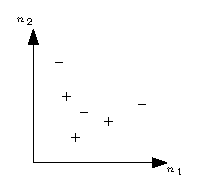
\includegraphics[width=0.25\textwidth]{images/N2_hypothesis_1.eps} 
\end{center}
We consider $H$ as the set of the functions that, assigns at all the points in a specific rectangle the $+$ value, and the $-$ value for all the points outside.
\begin{eqnarray*}
    h\in H \iff\Big( \exists R:=\{(x,y) \ : \ a\le x\le b\land c\le y\le d\} : h(x,y)=+\iff (x,y)\in R\Big )
\end{eqnarray*}
For that data samples, does not exists a consistent hypothesis, because does not exists a rectangle that contains all the $+$ value point, letting outside the $-$ value points.
\begin{center}
    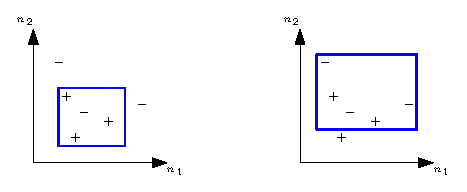
\includegraphics[width=0.6\textwidth]{images/N2_hypothesis_2.eps} 
\end{center}
If we consider the hypothesis space $H'=\mathcal P(H)$, geometrically, we can represent a function by a finite number of rectangles, in this case consistent hypothesis are allowed, but no $-$ value points can be predicted.
\begin{center}
    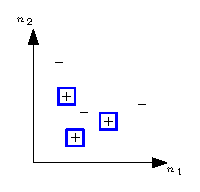
\includegraphics[width=0.25\textwidth]{images/N2_hypothesis_3.eps} 
\end{center}
Even in this example, a powerful representation of the hypothesis space lead to less generalization. This is known (as previously said) as \textbf{overfitting}, when the hypothesis space is not powerful enough, the problem could not be represented well, this is known as \textbf{underfitting}.\bigskip

If $n$ is a number that determines how big an hypothesis space, we can observe the following trend about the performance of a model.

\begin{figure}[h!]
    \centering
    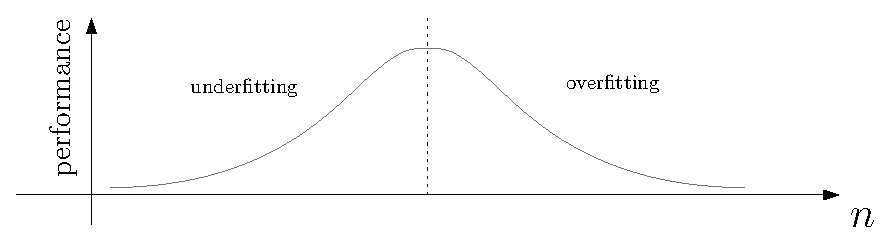
\includegraphics[width=0.65\textwidth]{images/fitting.eps}
    \caption{overfitting and underfitting trend}
    \label{img:fitting_trend}
\end{figure}

\subsection{Error Estimation and Performance Metric}
We want to define a metric for the performance of a model, to estimate how a given hypothesis $h$ is good respect to the others. We have to introduce some statistical methods, let's consider a target function\begin{equation}
    f:X\rightarrow Y
\end{equation}
where $Y$ is countable (classification problem). Let $\mathcal D$ to be a probability distribution over $X$.
\begin{definition}
    If $X$ is a countable subset of $\R^n$, $\mathcal D$ is a probability distribution on $X$ if\begin{eqnarray}
        \forall x\in X, \ \ \mathcal D(x)\in [0,1]
    \end{eqnarray}
    and \begin{align*}
        &\sum_{x\in X}\mathcal D(x)=1 
    \end{align*}
    if $X$ is an uncountable subset of $\R^n$,  $\mathcal D$ is a probability distribution on $X$ if \begin{eqnarray}
        \forall x\in X, \ \ \mathcal D(x)\ge 0
    \end{eqnarray}
    \begin{align*}
        &\int_X\mathcal D(x)dx=1
    \end{align*}
\end{definition}
\begin{definition}
    Given a target function $f:X\rightarrow Y$, an hypothesis $h$ and a probability distribution $\mathcal D$ on $X$, the \textbf{true error} is the probability that $h$ will misclassify an instance $x\in X$ drawn according to the distribution $\mathcal D$:
    \end{definition}
    \begin{equation}
        \text{error}_{\mathcal D}(h)=
        \Prob_{x\sim \mathcal D}
        (f(x)\ne h(x)) 
    \end{equation}
\textbf{Note}: With $x\sim \mathcal D$, we mean that $x$ was extracted from $X$ according to the probability distribution $\mathcal D$. We remind that, if $\mathcal D(x)=p$, then, the probability of extracting $x$ from $X$ by taking a random element is $p$.\bigskip

Since we can't compute $f$ for all $x\in X$, the true error can't be computed. We need to define an estimation of the error given by the sample set extracted from $X$.
\begin{definition}
    Given a target function $f:X\rightarrow Y$, an hypothesis $h$ and a sample (finite) set $\mathcal S\subset X$, the  \textbf{sample error} is defined as follows:
\end{definition}\begin{equation}
        \text{error}_{\mathcal S}(h)=
        \frac{1}{|\mathcal S|}\sum_{x\in\mathcal S}\delta(f(x)\ne h(x))
\end{equation}
where\begin{itemize}
    \item $\delta(\phi)=1$ if $\phi$ is true
    \item $\delta(\phi)=0$ if $\phi$ is false.
\end{itemize}
The sample error can be computed since, for each $x\in\mathcal S$, we know the value of $f(x)$. Is an approximation of the true error that depends from the sample set $\mathcal S$.\bigskip

Since $\text{error}_{\mathcal S}(h)$ depends from the choice of $\mathcal S$, is not fixed, but we can model it as a random process, by extracting $n$ random values from $X$ according to the distribution $\mathcal D$ to construct $\mathcal S$, and we can evaluate the expected value of $\text{error}_{\mathcal S}(h)$ denoted \begin{equation}
    \VA(\text{error}_{\mathcal S}(h)).
\end{equation}
We want to formalize this expected value, in this case the sample error is a random variable that assign to each subset $\mathcal S$ of $X$ of size $n$ a number between 0 and $1$:
\begin{align}
    &\text{error}_{\mathcal S}(h) : \Omega \rightarrow [0,1]\\
    &\Omega =\{\mathcal S \ : \ \mathcal S \subset X \land |\mathcal S|=n\}
\end{align}
in this context, $n$ is fixed. The probability of getting a certain value $\gamma$ from this random variable, is the probability to extract from $X$ a subset $\mathcal S$ of $n$ items such that, the sample error is $\gamma$, and this depends from the probability distribution $\mathcal D$ on $X$. The expected value $\VA(\text{error}_{\mathcal S}(h))$ is now well defined.
\subsection{Unbiased Estimation}
\begin{definition}
    The \textbf{bias} is defined as the expected value of the difference between the sample error and the true error:
\end{definition}
    \begin{equation}
        \VA(\text{error}_{\mathcal S}(h))-\text{error}_{\mathcal D}(h).
    \end{equation}
We want to find an unbiased sample error, in such case:\begin{equation}
    \text{bias = 0} \implies \VA(\text{error}_{\mathcal S}(h))=\text{error}_{\mathcal D}(h)
\end{equation}
To compute an unbiased estimation, we need to train an evaluate an hypothesis $h$ on different set, let $D$ to be the dataset, we have to split $D$ in two disjoint set\begin{align}
    &D=T\cup S\\
    &T\cap S = \emptyset
\end{align}
Usually, $\frac{|T|}{|D|}\simeq \frac{2}{3}$.
We use $T$ to train our learning function to get $h$, and then, we calculate the sample error on $S$\begin{equation}
     \text{error}_{ S}(h)=
        \frac{1}{| S|}\sum_{x\in S}\delta(f(x)\ne h(x))
\end{equation}
is ideal to choose $T$ and $S$ such that they have similar probability distribution over the features, in this case the random variable $\text{error}_{ S}$ is an unbiased estimator for the true error $\text{error}_{ \mathcal D}$. 
\subsection{The Cross Validation Algorithm and others Performance Metrics}
There exists an algorithm to estimate the expected value of the sample error, more the dataset $D$ is large, more the estimation will be precise.
The algorithm \ref{alg:CrossVal} estimate the expected value of the error, with $L$ is denoted a fixed learning algorithm:\begin{itemize}
    \item $h=L(T)$, is the result of the learning algorithm $L$ applied on the training set $T$
\end{itemize}
\begin{algorithm}
    \caption{K-Fold Cross Validation}\label{alg:CrossVal}
    \begin{algorithmic}
    \Require $D$, $k$, $h$, $L$
    \State partition $D$ in $k$ disjoint sets $S_1,S_2\dots, S_k$
    \For{$i=1,2\dots,k$}
    \State $T_i\leftarrow  D\backslash S_i$
    \State $h_i\leftarrow L(T_i) $
    \State $\delta_i = \text{error}_{S_i}(h_i)$
    \EndFor
    \State\Return $\text{error}_{L,D}=\displaystyle\frac{1}{k}\sum_{i=1}^k\delta_i$
    \end{algorithmic}
\end{algorithm}
We define the accuracy of a learning algorithm $L$ as \begin{equation}
    \text{accuracy}=1-\text{error}_{L,D}.
\end{equation}
The cross-validation algorithm can be used to compare the accuracy of two different learning methods $L_a$ and $L_b$, as shown in algorithm \ref{alg:CrossVal_compare}.

\begin{algorithm}
    \caption{Accuracy Comparator}\label{alg:CrossVal_compare}
    \begin{algorithmic}
    \Require $D$, $k$, $h$, $L$
    \State partition $D$ in $k$ disjoint sets $S_1,S_2\dots, S_k$
    \For{$i=1,2\dots,k$}
    \State $T_i\leftarrow  D\backslash S_i$
    \State $h_a\leftarrow L_a(T_i) $
    \State $h_b\leftarrow L_b(T_i) $
    \State $\delta_i = \text{error}_{S_i}(h_a)-\text{error}_{S_i}(h_b)$
    \EndFor
    \State\Return $\bar\delta=\displaystyle\frac{1}{k}\sum_{i=1}^k\delta_i$
    \end{algorithmic}
\end{algorithm}

Now that we defined the sample error, we can give a formal definition of overfitting. Let $h$  to be an hypothesis for a model, $h$ is overfitting is exists an hypothesis $h'$ such that\begin{align}
    &\text{error}_{S}(h)<\text{error}_{S}(h') \\ &\land\\
    &\text{error}_{\mathcal D}(h)>\text{error}_{\mathcal D}
\end{align}

Let's consider other performance metrics in binary classification. Let $f:X\rightarrow\{-,+\}$ to be the target function ad let $D$ to be a sample set such that, $90\%$ of elements in $D$ is of class $+$. An hypothesis that always returns $+$ will have an accuracy of $90\%$, in this scenario the dataset is unbalanced, so the accuracy is not a good performance metric for the model. We can consider a table that counts the number of points in the sample set that are well classified or misclassified by an hypothesis:\begin{center}
    \begin{tabular}{c|cc|}
\cline{2-3}
                                 & \multicolumn{2}{c|}{predicted class}                 \\ \hline
\multicolumn{1}{|c|}{true class} & \multicolumn{1}{c|}{+}              & -              \\ \hline
\multicolumn{1}{|c|}{+}          & \multicolumn{1}{c|}{true positive}  & false negative \\ \hline
\multicolumn{1}{|c|}{-}          & \multicolumn{1}{c|}{false positive} & true negative  \\ \hline
\end{tabular}
\end{center}
we can define two additional metrics that is useful when we deal with binary classification:\begin{itemize}
    \item the \textbf{recall} is the ability of the hypothesis to avoid false negatives and is defined as follows\begin{equation}
        \frac{\text{true positive}}{\text{true positive}+\text{false negative}}
    \end{equation}
    \item the \textbf{precision} is the ability of the hypothesis to avoid false positives and is defined as follows\begin{equation}
        \frac{\text{true positive}}{\text{true positive}+\text{false positive}}
    \end{equation}
\end{itemize}
the importance of these metrics depend on the application.
\bigskip
\begin{figure}[h!]
    \centering
    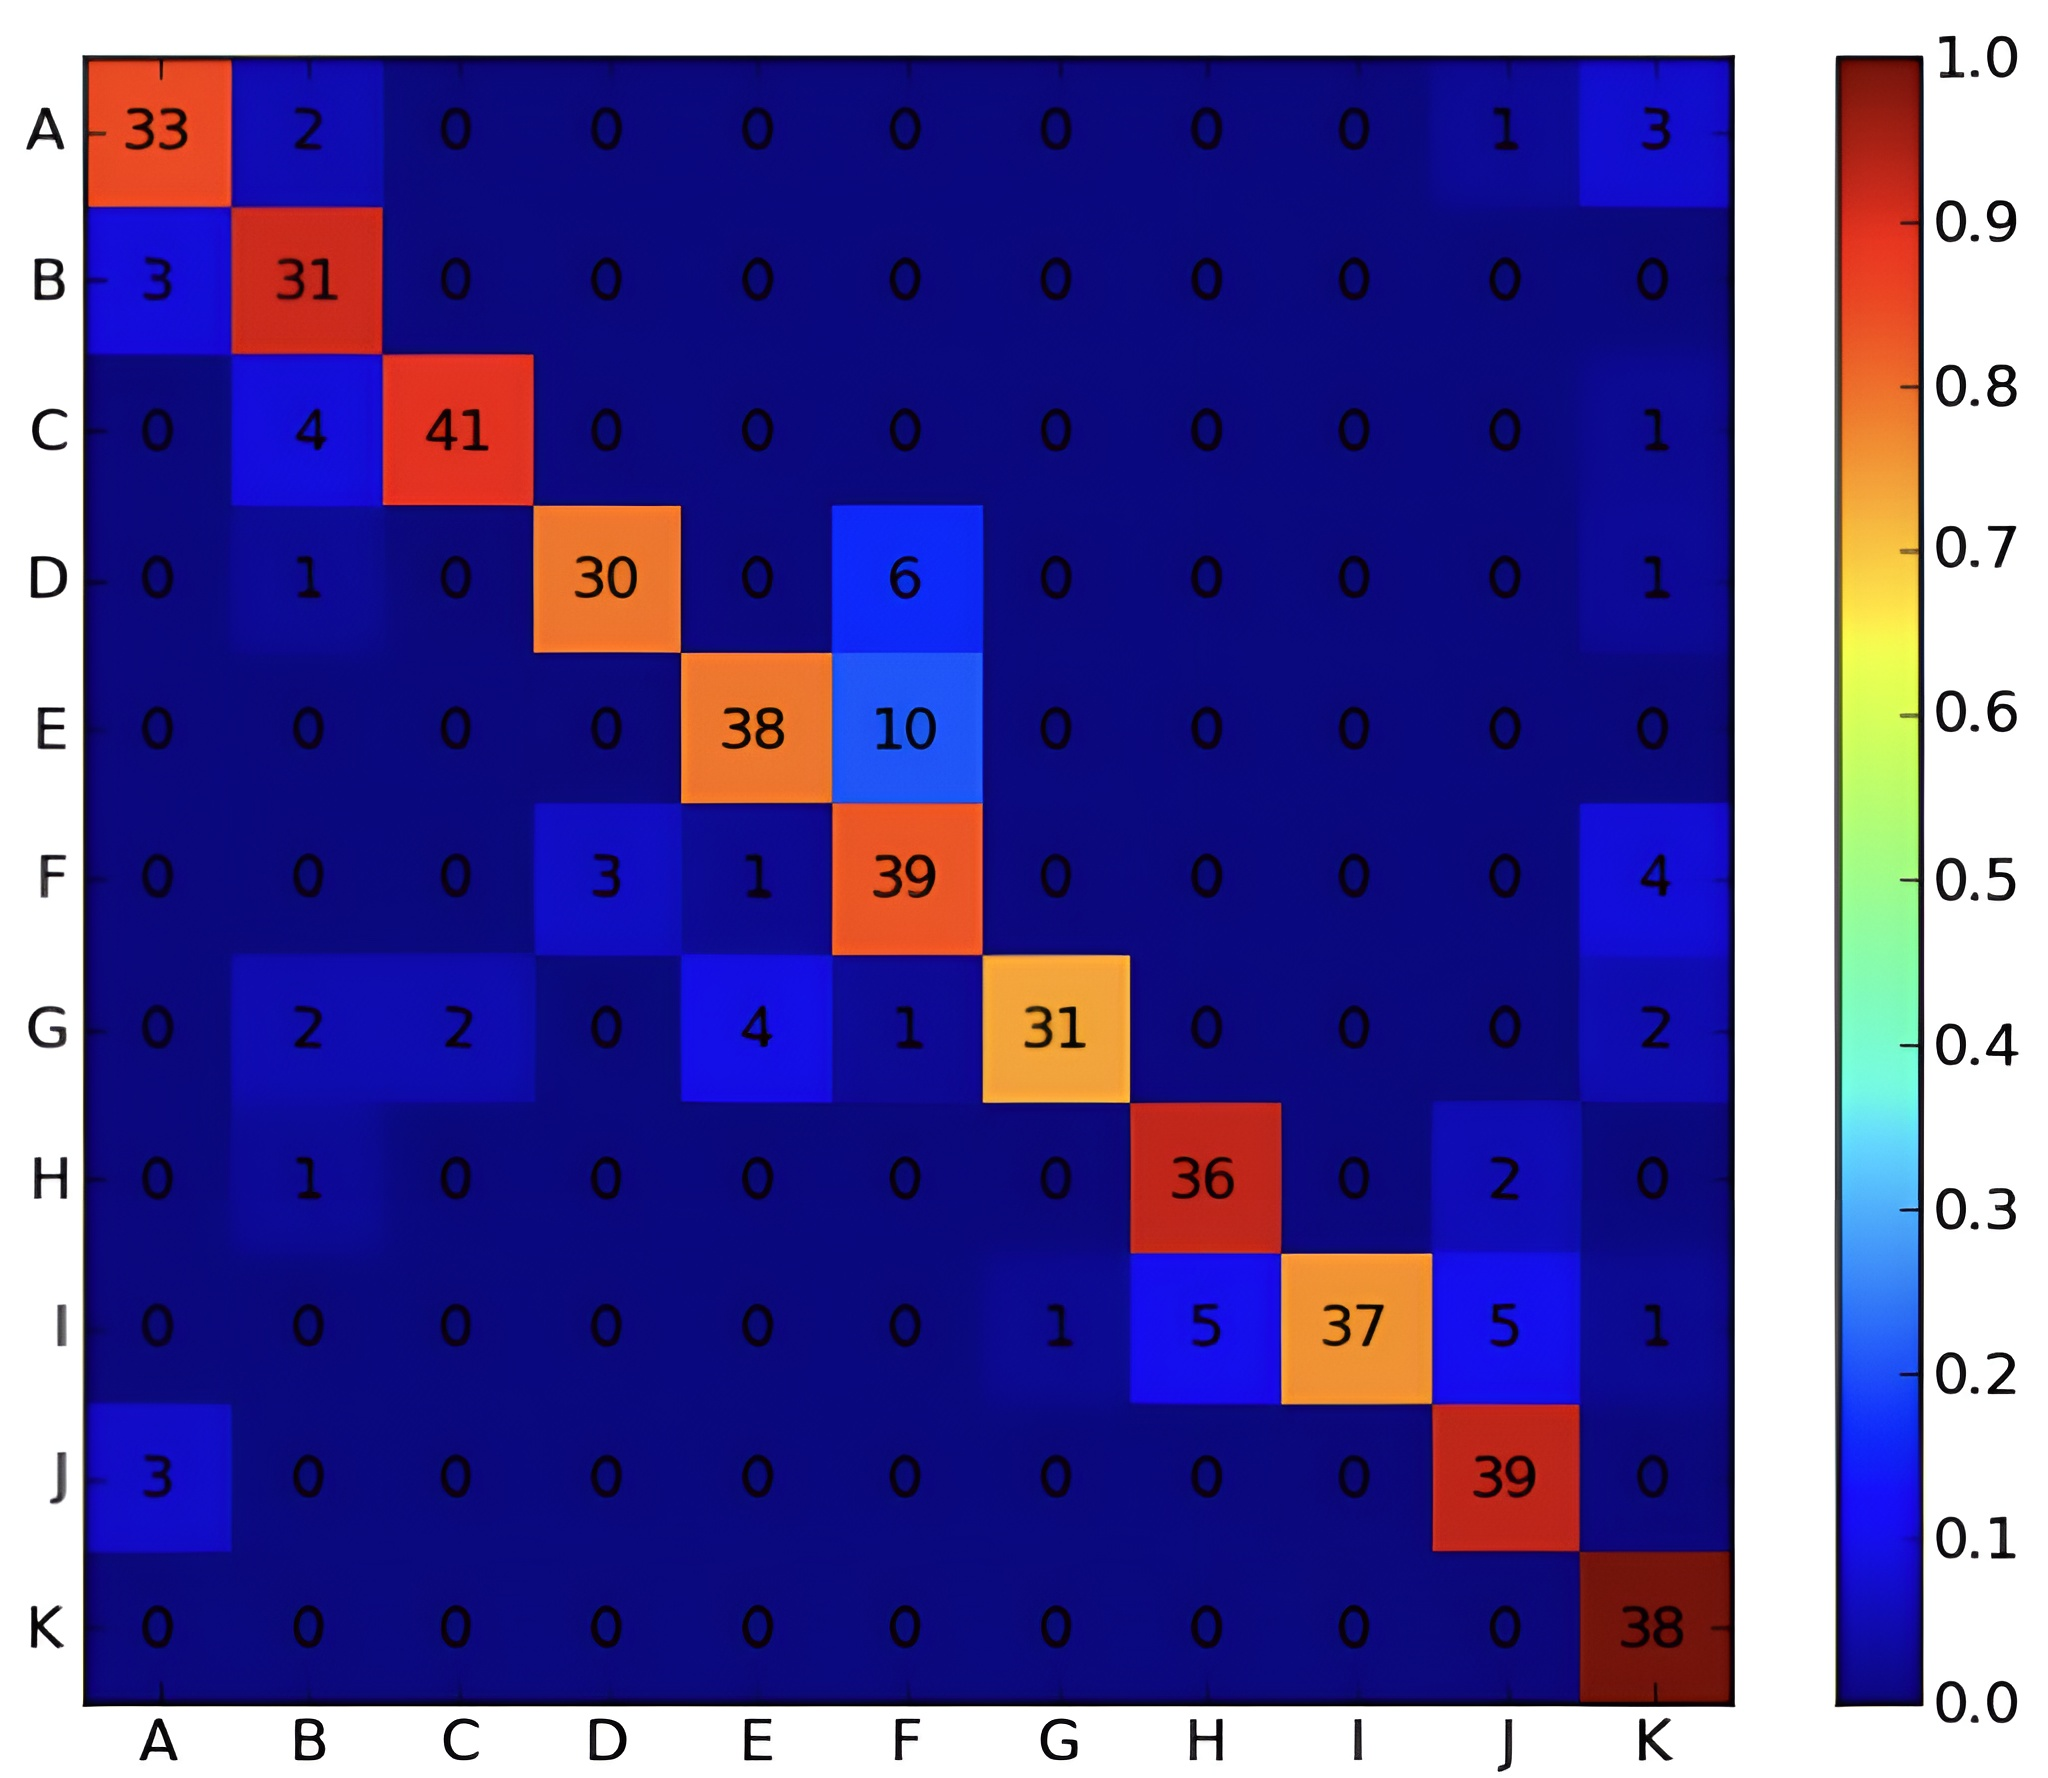
\includegraphics[width=0.3\textwidth]{images/conf_matrix.png}
    \caption{an example of a confusion matrix}
    \label{img:conf_matrix}
\end{figure}\bigskip

For the classification problems we can define an extension of the previous table, called \textbf{confusion matrix}, and report how many instances of class $C_i$ are classified in class $C_j$, the main diagonal contains the accuracy for each class. An example is shown in figure \ref{img:conf_matrix}.\bigskip

We consider now some performance metrics for the regression problems. Let $f:X\rightarrow\R^d$ to be the target function, and let $\hat f$ to be the learned function, for each sample $(x_i,f(x_i))$ in the dataset, we can compute the euclidian distance\begin{equation}
    |\hat f(x_i)-f(x_i)|.
\end{equation}
Let $n$ to be the number of samples, the three main metrics are the following:\begin{itemize}
    \item Mean Absolute Error\begin{equation}
        MAE=\frac{1}{n}\sum_{i=1}^n|\hat f(x_i)-f(x_i)|
    \end{equation}
    \item Mean Squared Error\begin{equation}
        MSE=\frac{1}{n}\sum_{i=1}^n(\hat f(x_i)-f(x_i))^2
    \end{equation}
    \item Root Mean Squared Error\begin{equation}
        RMSE=\sqrt{MSE}
    \end{equation}
\end{itemize}

The cross validation algorithm can be extended for the regression problems as shown in algorithm \ref{alg:CrossVal_regression}.

\begin{algorithm}
    \caption{K-Fold Cross Validation for Regression}\label{alg:CrossVal_regression}
    \begin{algorithmic}
    \Require $D$, $k$, $h$, $L$
    \State partition $D$ in $k$ disjoint sets $S_1,S_2\dots, S_k$
    \For{$i=1,2\dots,k$}
    \State $T_i\leftarrow  D\backslash S_i$
    \State $h_i\leftarrow L(T_i) $
    \State $\delta_i = MAE_{S_i}(h_i)$
    \EndFor
    \State\Return $\text{error}_{L,D}=\displaystyle\frac{1}{k}\sum_{i=1}^k\delta_i$
    \end{algorithmic}
\end{algorithm}
\end{document}